\section{Basic SPH Projection}

As noted in the introduction, there are many ways to project SPH data. The most common approach uses a pre-projected version of the kernel and for each particle loops over all pixels, calculating the kernel contribution from each particle to each pixel. It is important to ensure that the projected kernel corresponds directly to the same kernel used in the simulation, projected along one axis, to get the most accurate reconstruction. Here, for simplicity, we ignore the limb-brightening effects associated with this and simply use the two-dimensional version of the Wendland-C2 kernel,
\begin{equation}
  W(r, h) = C \cdot \max\left[\left(1 - \frac{r}{h}\right)^4 \left(1 + 4 \frac{r}{h}\right), 0\right],
  \label{eqn:kernel}
\end{equation}
with $r$ the inter-particle separation (or here the separation between the pixel sampling point and the particle), and $h$ the smoothing length of the particle. We take the ratio between the smoothing length and kernel extent $H/h = 1.897367$, and $C=7/\pi$ in accordance with \cite{Wendland1995, Dehnen2012}\footnote{The specific implementation of the kernel used here is defined in {\tt swiftsimio.visualisation.projection\_backends.kernels}.}.

\begin{figure}
  \centering
  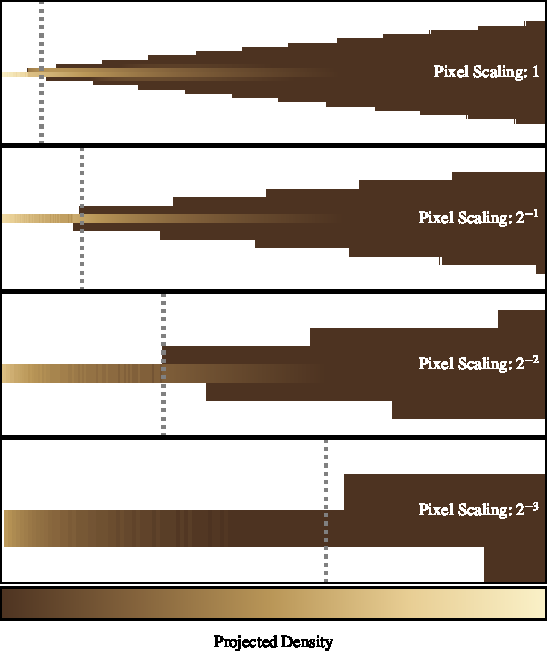
\includegraphics[width=\columnwidth]{./plots/gradient/gradients.pdf}
  \caption{Projected densities of a line of particles with a linearly increasing smoothing length. White pixels correspond to areas with exactly zero density (i.e. these pixels are not reached by the kernel extent of the particles). Each panel shows a different grid resolution, with the top containing 1095 pixels in the horizontal direction, the second row 547, and so on. The left hand side, where the pixels are much larger than the kernel extent of the particles, shows striped patterns as the uncorrected visualisation method struggles to capture the smooth gradient with such poor sampling. The pixels have been stretched vertically to more clearly display the gradients. The grey dotted line shows where the kernel extent of the particles is approximately equal to half a pixel width.}
  \label{fig:gradient}
\end{figure}

Algorithmically, such a scheme (described below as `Original') looks like:
\begin{enumerate}
  \item Start with a pixel grid full of zeroes, with the pixels of size ${\rm d}x$ along one axis.
  \item If the particle has a kernel extent $H < 0.5 {\rm d}x$, add all of its contribution onto the nearest cell centre, as this particle is `unresolved', otherwise:
  \begin{enumerate}
    \item Take all particle positions $\mathbf{r}_{\rm part}$ and particle  smoothing lengths $h$, and find which pixels this cell overlaps.
    \item Loop over the cell centers, $\mathbf{r}_{\rm pix}$ and evaluate the projected kernel $W(|\mathbf{r}_{\rm part} - \mathbf{r}_{\rm pix}|, h)$.
    \item Add this contribution onto the value of each pixel.
  \end{enumerate}
\end{enumerate}

In Fig. \ref{fig:gradient} we demonstrate this algorithm at various grid resolutions on a line of (3D) particles, projected into 2D. These are generated, from left to right, starting at an inter-particle separation of $10^{-4}$ in units of the box length, linearly increasing to $10^{-2.5}$. The smoothing length $h$ of the particles is set to be the same as the inter-particle separation.

In Fig. \ref{fig:gradient} the grey dotted line denotes the region where $H \approx 0.5 {\rm d}x$. The banding pattern to the left of this line is not a compression artefact, rather
it is the result of treating particles at this grid resolution as Monte Carlo
tracers of the field. Here, the particle spacing is approximately the same as the grid size, and so we expect the shot noise to be significant (with one or two sampling points in each pixel, the shot noise is of order 100\%). As the density increases, particularly for the larger pixels in the bottom panel, the signal to noise ratio increases and the smooth gradient is again recovered.

There is no excuse for the poor reconstruction of this smooth gradient; the problem demonstrated here is purely static. We have simply chosen to throw away everything we know about the smoothness of the field at a specific grid size and as a result have been penalised with significant reconstruction errors. This method, as we will demonstrate later, does converge to the correct answer when all particles are well resolved by the grid, but for some applications grids of that size are prohibitive and large pixel sizes (relative to the particle spacing) may be required for direct comparison to real-world observations.